

\documentclass{article}[14pt, oneside, a4paper, times]

\usepackage[utf8]{inputenc}
\usepackage[english]{babel}
\usepackage[T1]{fontenc}
\usepackage{epsfig}           % para incluir figuras
\usepackage{subfig}
\usepackage{graphicx}
\usepackage{setspace}
\usepackage{vmargin}
\usepackage{algorithm}
\usepackage{algorithmic}
\usepackage{amsfonts} 
\usepackage{amssymb}


\setpapersize [portrait]{A4}
\setmarginsrb {30mm} % margem esquerda
              {10mm} % margem topo
             {30mm} % margem direita
            {20mm} % margem pé
           {2ex}  % altura do espaco para cabeçalho
           {5ex}  % espaço entre fim do cabeçalho e início do texto
          {0pt}  % altura do espaço para rodapé
         {20mm}  % espaço entre fim do texto e fim do rodapé

\doublespacing

%=======================================================================
\pagestyle{myheadings}
\begin {document}

\title{Classifier Combination and Feature Extraction 
\\ \large Concavity Features}
\author{Luiz S. Oliveira and Marisa Morita  
\\
\vspace {-10pt}
Federal University of Parana (UFPR)\\
\vspace {-10pt}
Department of Informatics (DInf)\\
\vspace {-10pt}
R. Rua Cel. Francisco H. dos Santos, 100, Curitiba, PR, Brazil \\
lesoliveira@inf.ufpr.br \\ 
}


\date{}
\maketitle
%\vspace{-2\baselineskip}
\thispagestyle{empty}

%\begin{abstract}

%bla bla


%\end{abstract}

%%%%%%%%%%%%%%%%%%%%%%%%%%%%%%%%%%%%%%%%%%%%%%%%%%%%%%%%%%%%%%%%%%%%%%%%%%%%%%%%%
% Introduction 
%%%%%%%%%%%%%%%%%%%%%%%%%%%%%%%%%%%%%%%%%%%%%%%%%%%%%%%%%%%%%%%%%%%%%%%%%%%%%%%%%
\section{Introduction} 

In the previous reports we have introduced a feature set based on global features and reported the performance of this feature set using three different architectures of HMMs to recognise handwritten month words. In this report we performed some experiments to combine those three architectures and also implemented a new feature set based on concavity information. 

The source code for this new feature set is available in the SVN repository. Before compiling the code make sure to update the \textsf{PPROJ} variable in the \textsf{Make\_orand\_concfeat} file available in the directory \textsf{./tools/orand/batch/feature/gen} and also to update the defines in the \textsf{global.h} file, available in the directory \textsf{./tools/orand/inter/include}. To compile the source code use

\begin{verbatim}
make -f Make_orand_concfeat
\end{verbatim}

\noindent And to execute the program, type

\begin{verbatim}
./orand_globfeat feat2 concf
\end{verbatim}

The program generates three different files for training, validation and testing, respectively. Those files are located in the directory \textsf{./tools/orand/param/feature/feat2/concf/vq} 



\section{Combining Classifiers}


A classical strategy for constructing classifiers is to evaluate different models and topologies in order to select the one with the highest performance with respect to a testing data set. However, the construction of a universal classifier that performs an appropriate classification for any kind of input is a utopian goal. Ranawana \cite{Ranawana06} states that, frequently, the construction of an ideal classifier for a certain application is almost impossible. An interesting alternative to deal with the aforementioned problem is the construction of multiple-classifiers based systems. In this approach, many classifiers produce independent decisions, which are then combined to yield a final response (the estimated class). In fact, starting from the assumption that different kinds of classifiers allow us to classify accurately different patterns, a combination of these classifiers may achieve more accurate decision on the overall data set, instead of the performance achieved by only one classifier \cite{Brown05,Kuncheva03,Kittler98}.

With that in mind, we have performed some experiments to combine the three different HMM architectures reported in the previous report. However, we were conscious that the expected diversity may not be available since all the classifiers were trained with the same feature set. In  such a case, the only source of diversity would be the different architectures of the HMMs. In spite of that, we have implement and tested all the combination rules described by Kittler et al in \cite{Kittler98}. Table \ref{results:tab} shows the results of each HMM architecture and also the results os all combination rules.


\begin{table} [ht!]
\caption {Summary of the recognition rates obtained in the experiments}
\begin{center}
\begin{tabular}{ccc} \hline 
 \multicolumn{1}{c}{Experiment}&
 \multicolumn{1}{c}{Number of HMM Models} &
 \multicolumn{1}{c}{Rec. Rate (\%)} \\ \hline

I & 24 & 80.9 \\
II & 36 & 82.2 \\
III & 12 & 82.4 \\ \hline
Combinaton Rule & & \\ \hline
Voting &  & 82.0 \\
Max    &  &  82.5 \\
Sum    &  &  82.5 \\
Product&  &  82.2 \\ \hline


\end{tabular}
\label{results:tab}
\end{center}
\end{table}

As we may notice, the combination did not bring any improvement in terms of performance. The Sum and Max rules produced a recognition rate of 82.5\%, which is similar to the best classifier (82.4\%). Other rules, such as voting and Product, did not increase the recognition rate. The Product rule is effectively a severe rule of fusing the classifier outputs as it is sufficient for a single recognition engine to inhibit a particular interpretation by outputting a close to zero probability for it \cite{Kittler98}. In other words, if only one classifier produces a low score for a given testing pattern, the combination of all classifiers would be a low score, independently of the scores produced by the other classifiers.

It is worth of remark, though, that even not improving the recognition rate of the system, combining these different architectures certainly provide a more reliable system. In order to increase the diversity in our classification system, we have implemented another feature set, which is described in the next section.


\section{Concavity Features}

Concavity features have been successfully used as pattern representation for different handwriting recognition problems \cite{Liu03,Morita2004}. The basic idea of concavity measurements is the following: for each white pixel in the component, we search in 4-Freeman direction (Figure \ref{conc:fig}a), the number of black pixels that it can reach as well as which directions the black pixel is not reached. When black pixels are reached in all directions (e.g. point $x_1$ in Figure \ref{conc:fig}c), we branch out in four auxiliary directions ($s_1$ to $s_4$ in Figure \ref{conc:fig}b) in order to confirm if the current white pixel is really inside a closed contour. Those pixels that reach just one black pixel are discarded.

 \begin {figure} [htb]
    \centering
    \mbox
        {
        \subfloat[] {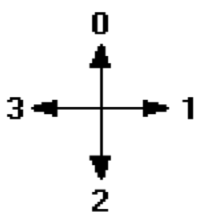
\epsfig {file=foura, width=2cm}}\quad 
        \subfloat[] {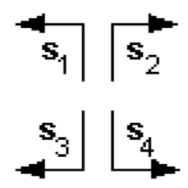
\epsfig {file=fourb, width=2cm}}\quad 
        \subfloat[] {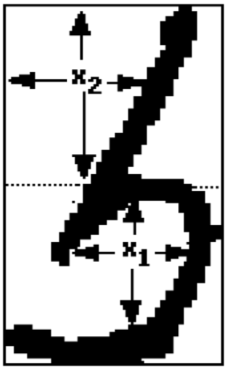
\epsfig {file=conc, width=2cm}} 
        }
    \caption{Concavity Features \cite{Morita2004}}
    \label{conc:fig}
\end{figure}


To reduce the feature vector as well as the handwriting variability, we are considering only the more relevant concavities. We are labelling the white pixels which have black pixels in three or four directions (five configurations). The white pixels with two or less directions are often located on the grapheme borders (e.g., point $x_2$ in Figure \ref{conc:fig}c). The labelling leads to a vector composed of nine components  for each grapheme: $s_1$ to $s_4$ and five configurations. Since we are zoning the grapheme into two equal parts along the vertical axis, the final feature vector contains 18 components normalised between 0 and 1. In order to use this feature vector to train the HMM-based classifier, it needs to be discretised using a vector quantisation technique. Such a technique is being implemented right now.

\section{Conclusions}

In this report we have reported the results of the experiments related to the combination of classifiers based on global features. We have seem that the diversity produced by the different HMM architectures was not enough to produce the diversity that could be exploited by the combination techniques. To mitigate this problem, we have implemented a feature set based on concavities. Since this representation creates a feature vector composed of continuous values, it will be discretised before training the HMMs. For the next report we expect to have the recognition rates produced by this new feature vector as well as the results of the combination of concavities and global features. 


\bibliographystyle{IEEEbib}
\bibliography{refer}



\end{document}



